%!TeX root = main.tex
\section{Report of 2024 05 02}



I finally have the particle collision detection software working. The number of collisions have been accurate and precise during substantial testing -  
the only negative is that it slowed the system down a bit. There is quite a bit that can be done to speed it up. 

I have enough to start flow regimes so I'll come back to performance afterwards. I want to put a load on it to see how it performs when the 
particles are moving and interacting. Plus, I don't fully understand the metrics I have. 

I need to review with you the performance testing so far and any feedback woud be appreciated.

\subsection{Performance}
The non-working version did 2 million in 17fps now it is down to 2 fps (comparing Table \ref{tab:V-Cube Performance Data} and Table \ref{tab:V-Cube Performance DataOld}).
I tested the collision detection performance for the number of particles where the cell density is 30 and the collision density is 0.5 (15 collisions per cell).
The results are listed in table \ref{tab:V-Cube Performance Data}.

I plotted frame per second vs number of particles \Figo{Perf_VCUBE01}. And I plotted seconds per frame vs number of particles \Figo{Perf_VCUBE02} which seems to be linear.


I also tested a fixed number of particles against a growing number of collisions per cell where density of collisions $(\frac{collsions}{cell}$) 
varied from 10\% to 100\% (100\% means 30 collisions per cell) \figo{Perf_RCPCD_Density001}. There was allot of variance but I suspect this is due to the randomness of the
CPU sending commands. Vulkan has no coordination or functionality for setting the frame rate - it renders frames as fast as the CPU will let it.
I can run the test a couple more times and compare the randomness to see if it remains stable.

I plotted linearity ($\frac{spf}{number particles}$) and something I labeled CCP ($\frac{number particles}{collisions}$). \q{I don't understand 
these but it's highly likely that I wrote them down wrong or just misunderstood from the the email.}

There is a fast degradation of performance especially from 4096 up to about 32000 particles. But the compute is not fully threaded nor is the graphics pipeline. 
There are eight sub threads still available for both. I suspect this is is a result of the increasing random access
due to larger and larger particle memory (See \figo{RandomVSequential}). The compute kernel is really throwing pointers around even though it is fully parallel. 
As I understand it, the random access degrades the L2 cache.

\Figo{GPUTrace} shows an NSight GPU trace for 117650 particles. If I am reading it right the compute phase takes 24.15ms while the graphics (vertex and fragment) are taking 0.57 ms- 42 times as long. They are doing close to the same amount of work. Something is broken here I suspect.

Other issues are 

\begin{enumerate}
\item There is only one buffer so the system can be built to be double buffered.
\item The compute kernel only determines collision response for the source particle (the one whose link list is being traversed). As each particle is tested for contact then each particle is responsible for updating only its information. So it does twice the work it needs to. Experiments with atomics are worthwhile since the loss of performance due to atomics may be less than doubling the kernel calls. 
\item Atomics are surprisingly fast. Broad detection on the graphics pipeline was 0.57 ms as it processed 117,650 particles.
\end{enumerate}

%\input{../images/RandomVSequential.tex}
%\input{../images/GPUTrace001.tex}
%\input{../images/GPUTrace.tex}
%\newpage
%\input{../tables/V-Cube Performance Data.tex}
%\newpage
%\input{../tables/V-Cube Performance Data001.tex}
%\newpage
%\begin{figure}[h]
\centering
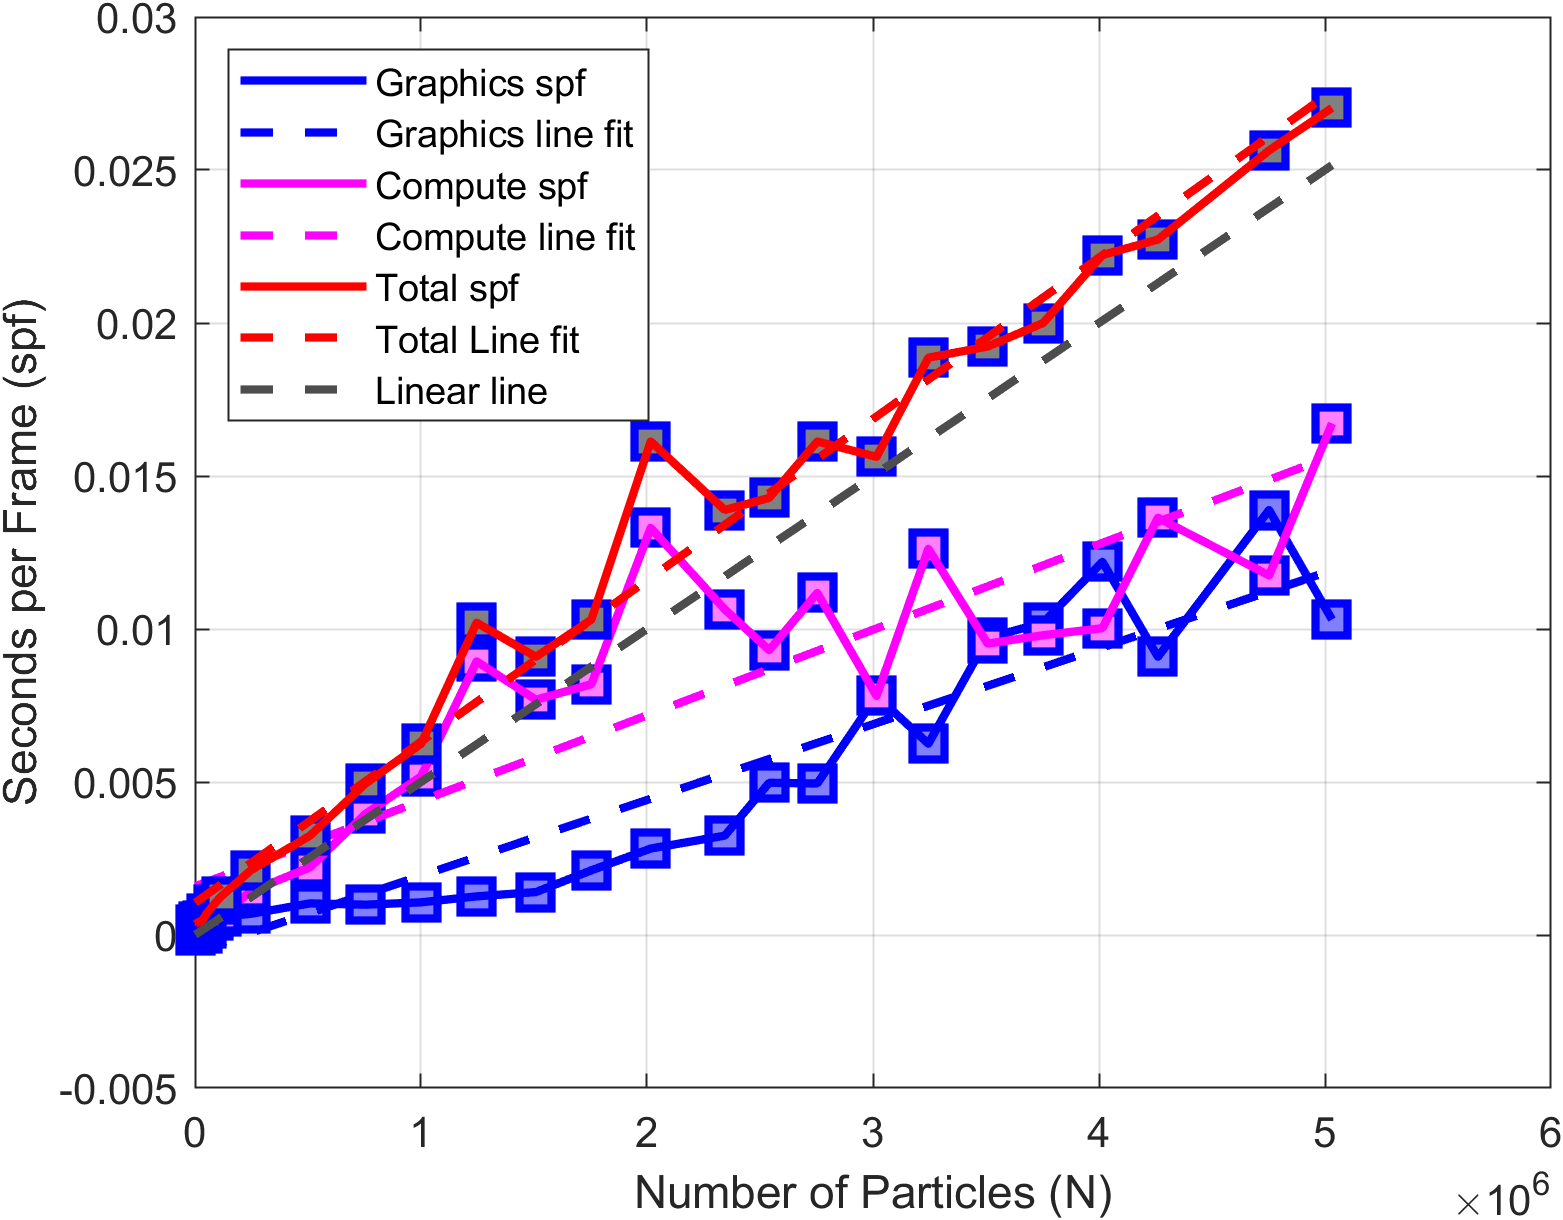
\includegraphics[width=2.97in]{../plots/Perf_VCUBE021.png}
\captionof{figure}[FPS Performance Data]{Seconds per frame for 0.5 collision density with 30 particles per cell verses number of particles.}
\label{fig:Perf_VCUBE02}
\end{figure}

%\begin{figure}[h]
\centering
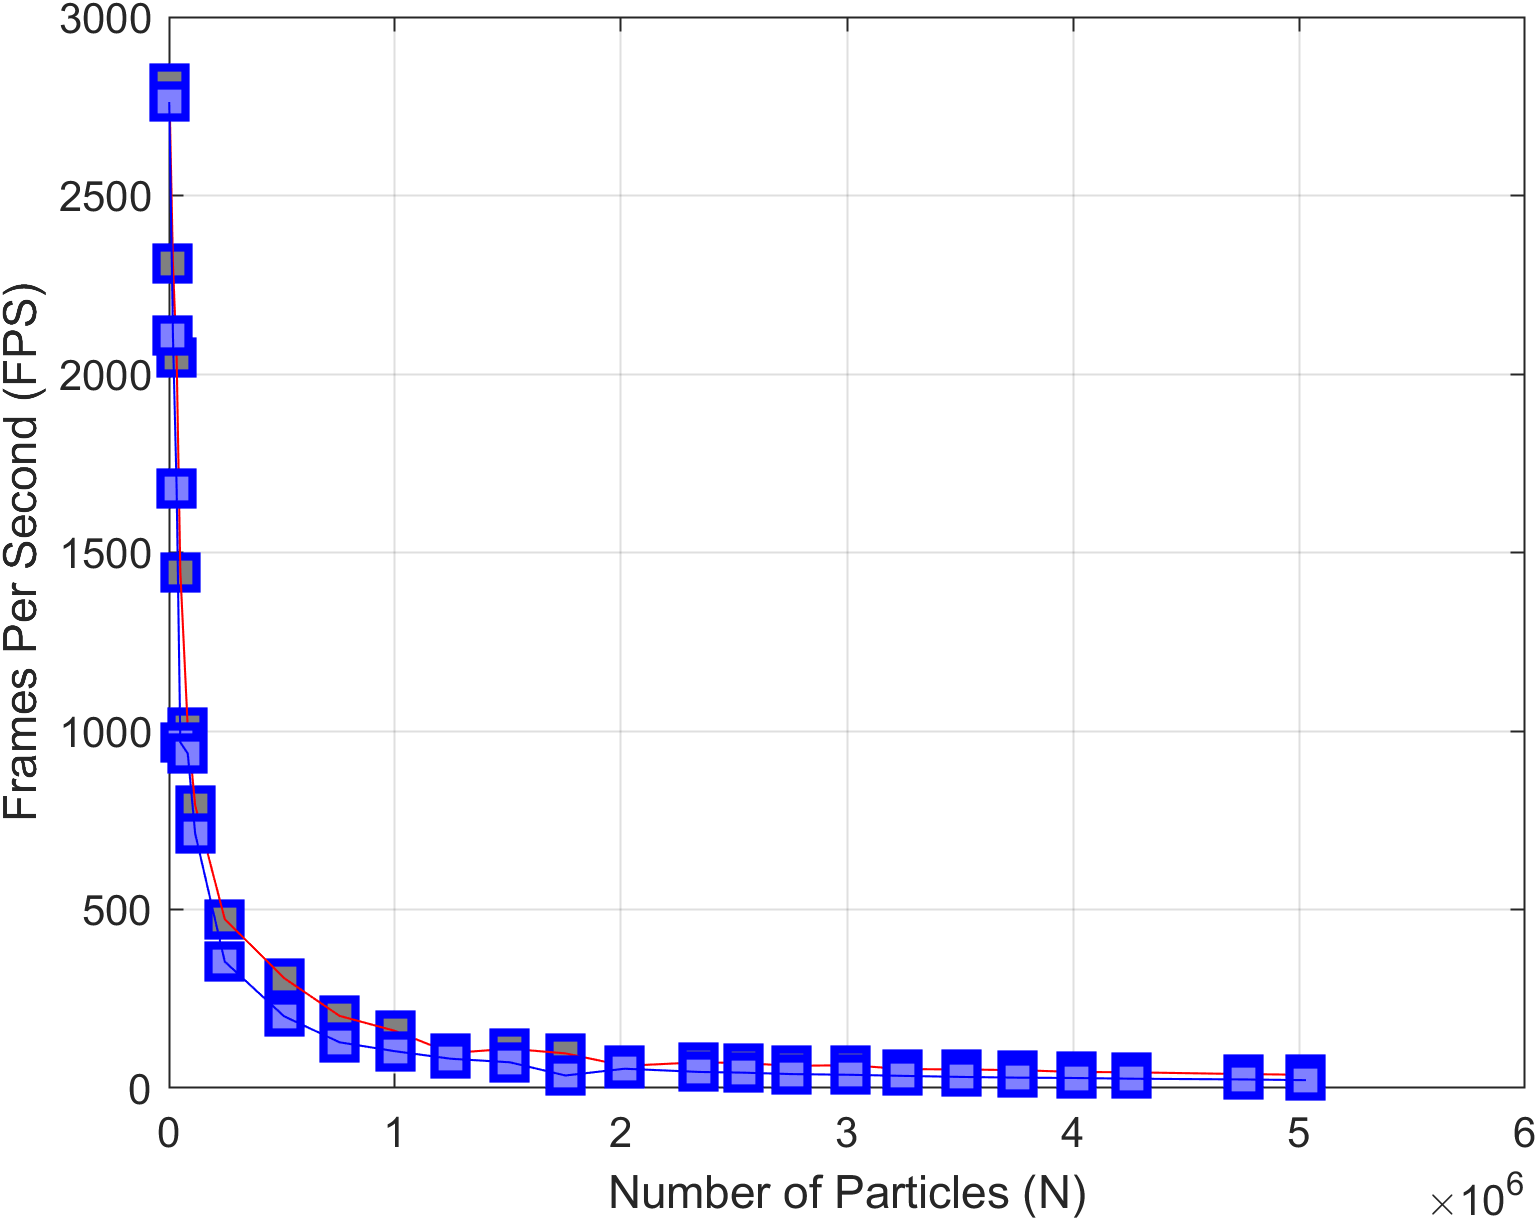
\includegraphics[width=2.97in]{../plots/Perf_VCUBE011.png}
\captionof{figure}[SPf Performance Data]{Frames per second for 0.5 collision density with 30 particles per cell verses number of particles.}
\label{fig:Perf_VCUBE01}
\end{figure}


%\begin{figure}[h]
\centering
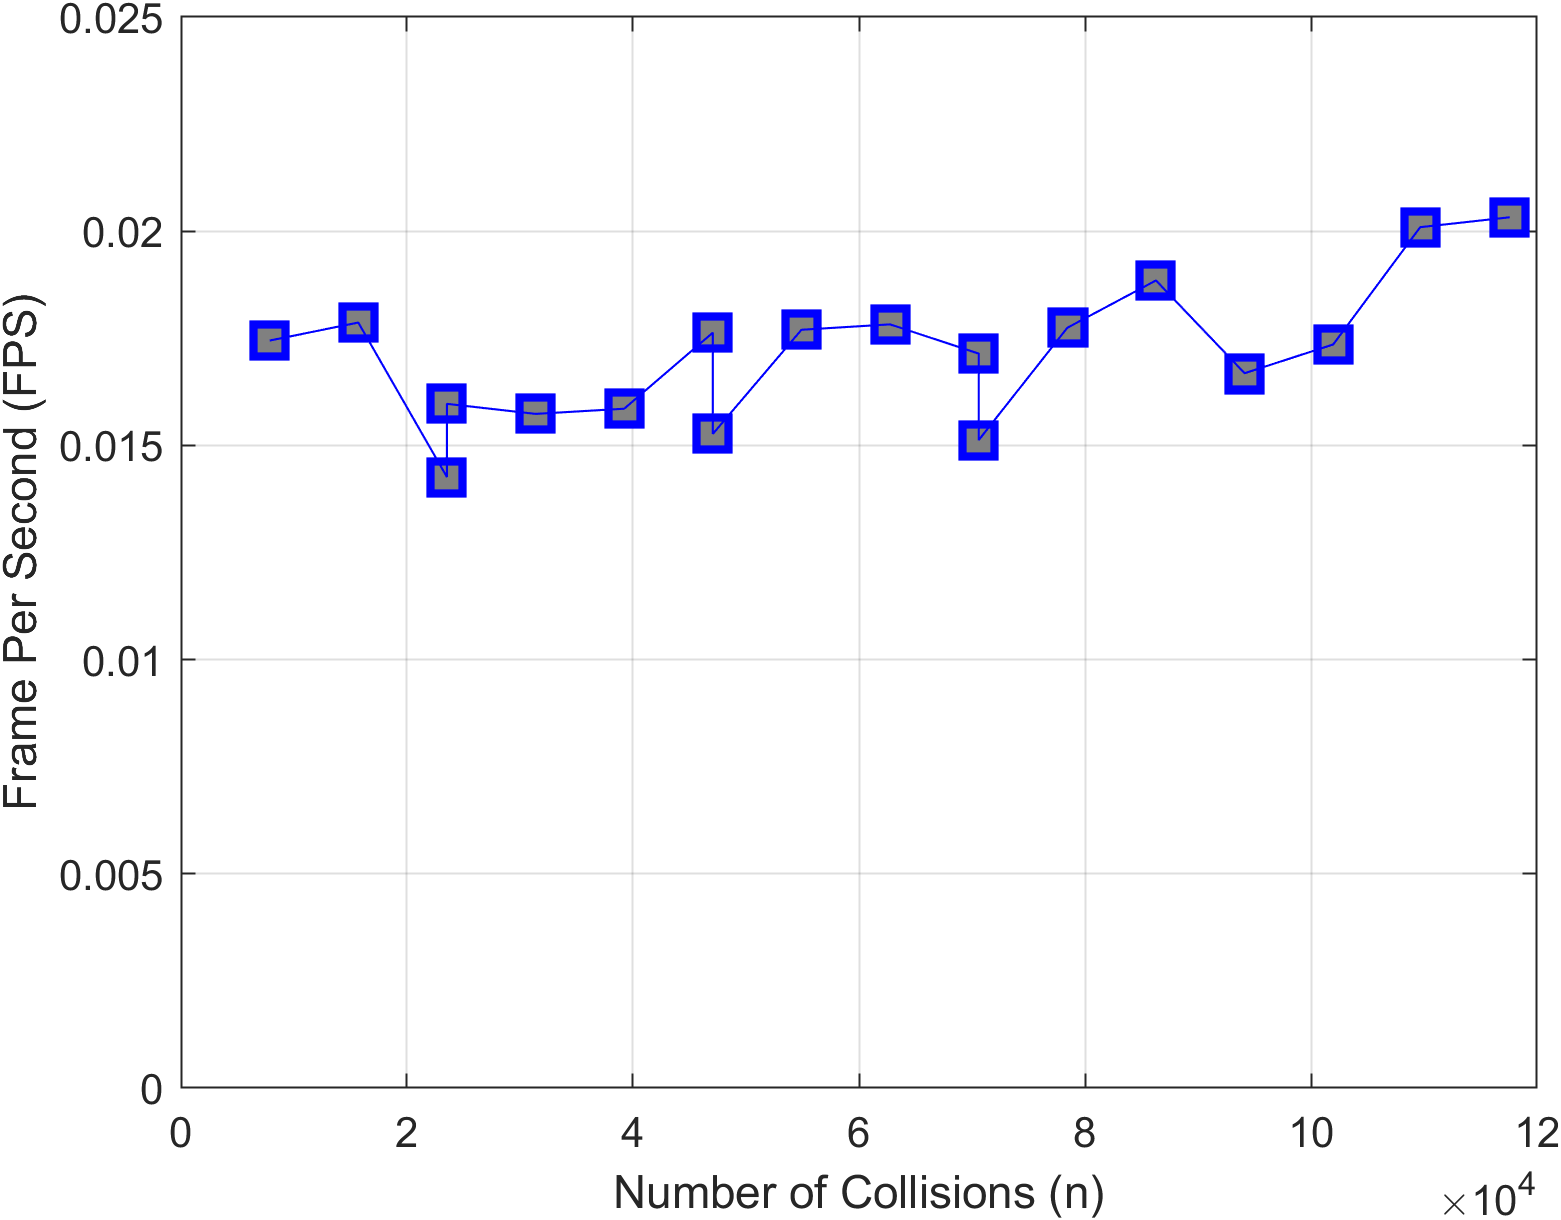
\includegraphics[width=2.97in]{../plots/Perf_RCPCD_Density0011.png}
\captionof{figure}[Frame rate verses density of collisions at 117,650 particles particles and density 0.1-1.0..]{Frame rate verses density of collisions at 117,650 particles and density from 10-100\%}
\label{fig:Perf_RCPCD_Density001}
\end{figure}

%
%\begin{figure}[h]
\centering
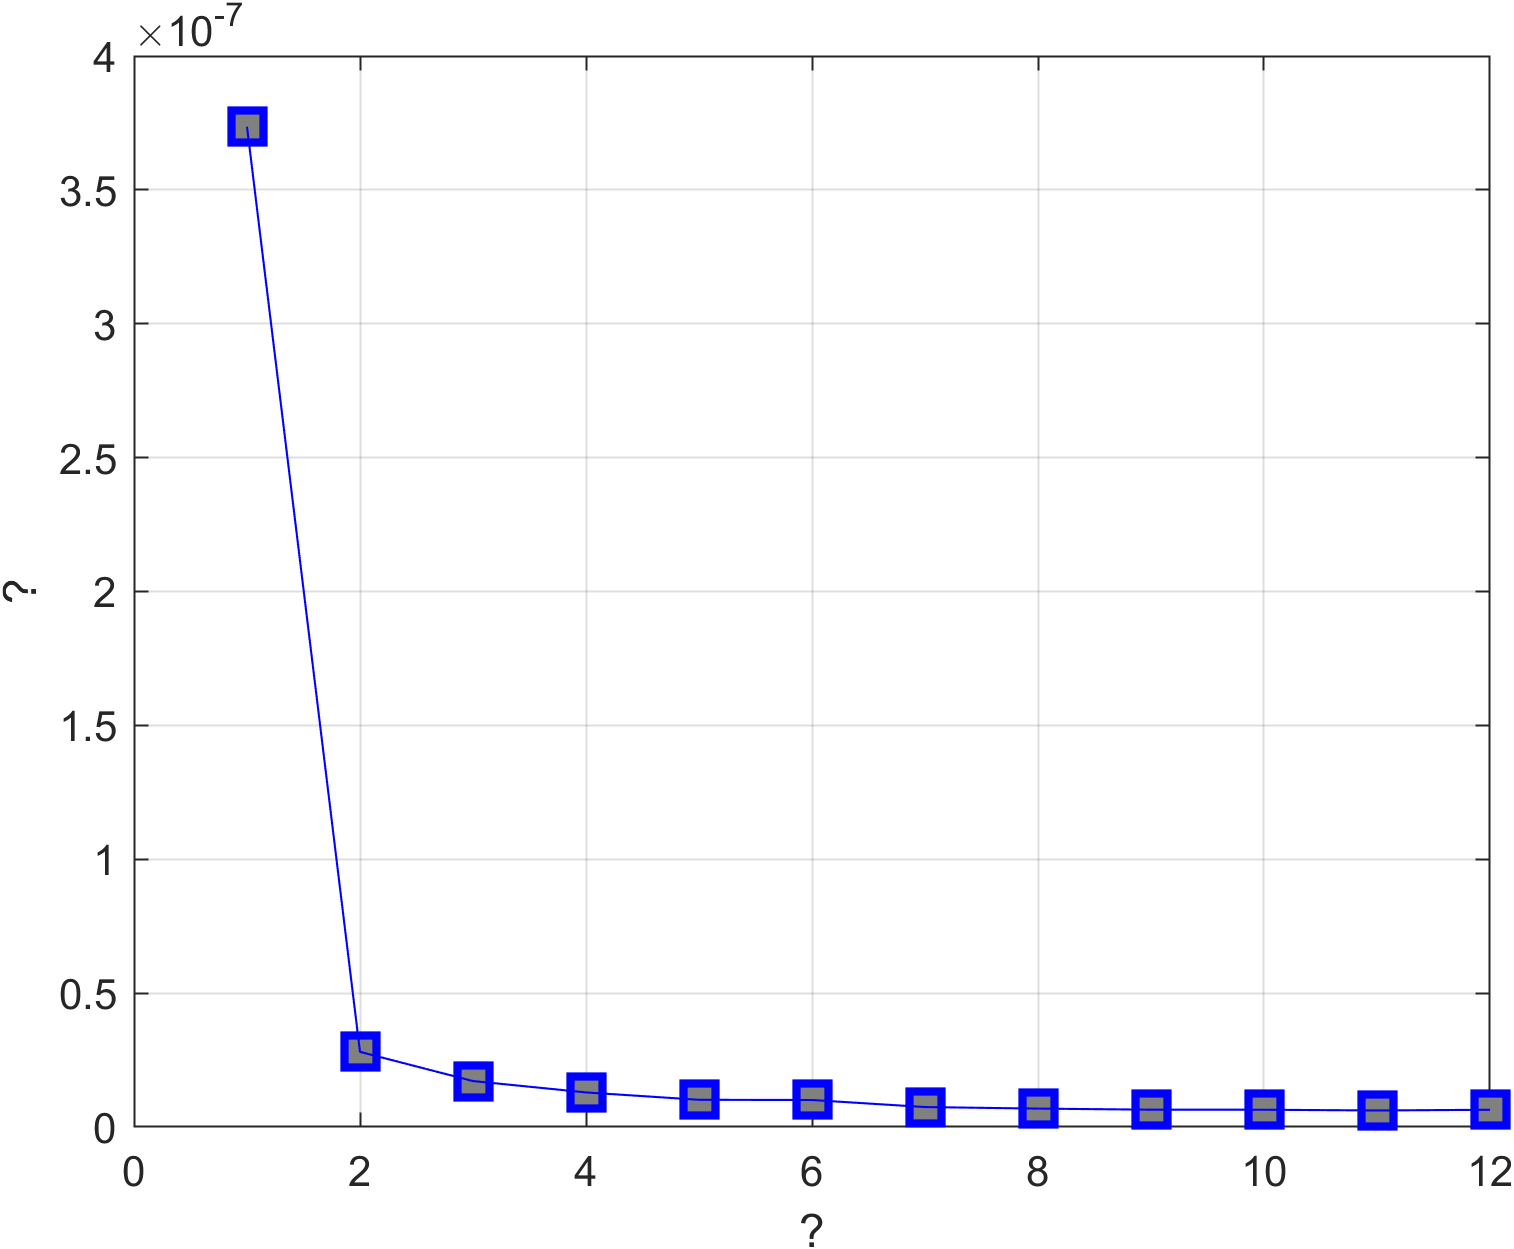
\includegraphics[width=2.97in]{../plots/Perf_VCUBE031.png}
\captionof{figure}[Linearity.]{Linearity - Frame time divided by number of particles for 0.5 collision density with 30 particles per cell verses number of particles.}
\label{fig:Perf_VCUBE03}
\end{figure}

%
%\begin{figure}[h]
\centering
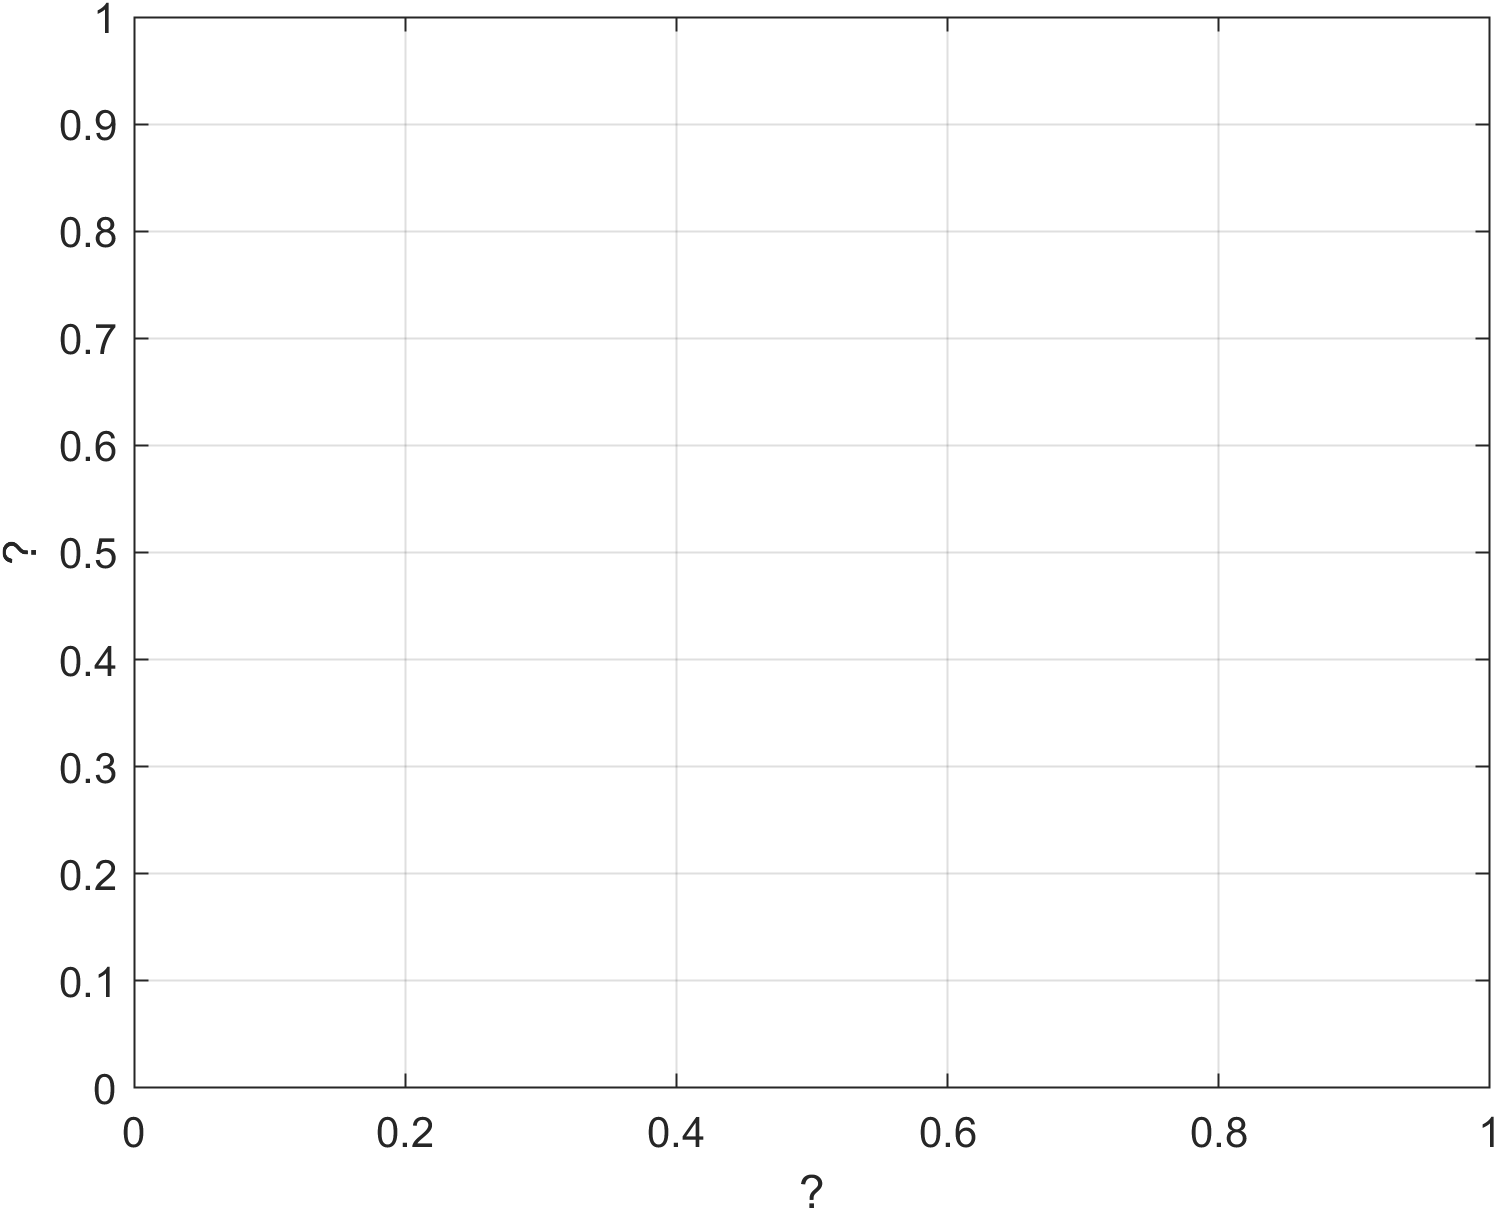
\includegraphics[width=2.97in]{../plots/Perf_VCUBE041.png}
\captionof{figure}[Frame time divided by number of particles.]{CCP number of collisions divided by number of particles for 0.5 collision density with 30 particles per cell verses number of particles.}
\label{fig:Perf_VCUBE04}
\end{figure}

%Fig. \ref{fig:Perf_RCPCD_Density001}

